% ************ Capítulo 1 ************
%\renewcommand{\chaptername}{Capítulo}
\chapter{Introdução}
\label{cap:1}

\section{Enquadramento}
A reciclagem de residuos de velas ainda não é neste momento uma ativadade com grande expressão no mercado Português. 

\section{Apresentação da empresa}
\todo{Falar sobre a empresa}
A Natural Life, Lda. é uma empresa fundada em 2013. Está sediada na rua de terramonte nº 781, Armazém C20, na Maia. Tendo como atividade a recolha e reciclagem de resíduos de velas, a Natural Life surge como uma empresa ecológica, inteiramente ligada a área Ambiental, mais concretamente à Reciclagem.\cite{NaturalLife}\\
A recolha da informação da empresa era feita por meio de uma base de dados desenvolvida com o software Microsoft Access\label{sym:MS_ACCESS} com auxilio de alguns formulários embutidos na mesma. Aquilo que se previa ser uma solução temporária, acabou por se tornar definitiva pela simplicidade que a interface oferecia aos utilizadores, pela simples integração com outras aplicações Microsoft, como o Microsoft Excel\label{sym:MS_EXCEL} e Microsoft PowerBI\label{sym:MS_POWERBI}, e pela dificuldade de encontrar um sistema ERP\label{sym:ERP} comercial com as características da solução temporária, com um custo de aquisição que a empresa pudesse comportar e permitisse obter interfaces simplistas para os utilizadores que já se tinham acostumado com os formulários em Access.
A solução desenvolvida em Access é bastante limitada no que toca a executar o mesmo ficheiro em dois computadores ao mesmo tempo, o que limitava as opções da administração nos seus planos expansão da fábrica. Este constrangimento obriga os colaboradores a deslocar-se vários metros até ao único computador da fábrica, onde a base de dados estava, para aí fazerem registos. Esta situação impede ainda que possam ser consultados registos durante o dia, em outro computador, que não o computador da fábrica. Por fim esta base de dados não suporta níveis de acesso, o que quer dizer que qualquer pessoa com acesso ao computador poderá não só ver todos os registos da empresa como modificá-los ou até mesmo apagá-los.\\
Assim, pretende-se com este projeto de estágio a implementação de um novo sistema de recolha e consulta de informação, desenvolvido pelo aluno e consequente migração dos dados anteriormente registados.
\newpage
%%%%%%%%%%%%%%%%%%%%%%%%%%%%%%%% Ainda tem de ser feiro %%%%%%%%%%%%%%%%%%%%%%%%%%%%%%%%%%
% \section{Motivação}
% \todo{Fazer}




\section{Objetivos}
Desenvolver um sistema de informação (SI\label{sym:SI}), de raiz, para efetuar o registo da informação gerada na fábrica. Este SI seria composto por uma secção protegida para a analise da informação registada e teria ainda de permitir uma fácil integração com as ferramentas Microsoft Excel e Microsoft PowerBI.

%%%%%%%%%%%%%%%%%%%%%%%%%%%%%%%% Ainda tem de ser feiro %%%%%%%%%%%%%%%%%%%%%%%%%%%%%%%%%%
\section{Calendarização}
No Diagrama de Gantt a seguir é descrito as fases do projeto e a sua respetiva duração.

\begin{figure}[htbp] 
    \begin{center}
    % Requires \usepackage{graphicx}
    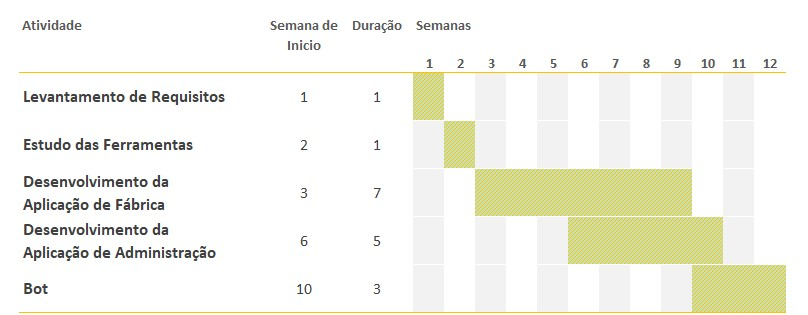
\includegraphics[width=\textwidth,keepaspectratio]{figuras/DiagramaGant.jpg}
    \caption{Gantt chart com o plano de trabalhos de PROES\label{sym:PROES}}\label{fig:gantt chart} 
    \end{center}
\end{figure}

\section{Organização do relatório}
No Capítulo 1 é feito o enquadramento do projeto dando uma visão superficial do projeto
\newline\newline
No capítulo 2, são apresentados o estado d'arte sobre a realidade da empresa antes do inicio do projeto, soluções disponíveis no mercado e objetivo global do projeto.
\newline\newline
No capítulo 3, é apresentada a lista de requisitos e a proposta global dos diferentes componentes do sistema.
\newline\newline
O capítulo 4, destina-se à descrição do desenvolvimento e implementação do projeto, apresentando em detalhes as características do trabalho desenvolvido.
\newline\newline
No capítulo 5, são descritos os resultados da implementação e o \textit{feedback} geral recebido pela administração e pelos colaboradores da empresa.
\newline\newline
No último capítulo, o 6º, são apresentadas as conclusões do projeto, incluindo nestas a opinião crítica do estudante face ao trabalho desenvolvido.
